\chapter{Routing}

Even nowadays the routing is often done manually for analog circuits. This is mainly caused by a lack of good tools and consequently the missing trust of engineers in them. The engineers consider a lot of different constraints during the routing, for example symmetries, net lengths and capacitive couplings. All these things have a major impact on the performance of the circuit, as it is very important in the analog world to have a really accurate signal level because only high or low isn't enough.

Additonally, the designer adds guards and rings to the placement to protect certain devices from noise. This noise can come for instance from the clock net or other routes, which carry a signal with high frequency. But high frequencies aren't the only disturbing effects, already during the placement the designer has to consider temperature gradients, caused by transistors with a high power consumption. To avoid problems with different temperatures in the substrate of for example the devices of a differential pair they can be placed symmetric or can even have a common centroid. Around these grouped modules the designer then can create a guard ring to protect the devices even more. An example for a manually routed layout can be seen in \nref{fig:miller_amplifier_routed_layout}.

So for an automatic routing algorithm a lot of different constraints must be considered. There are even more obstacles than just the devices and already created routes, for instance the routes should pass over guard rings. To solve this problem in the following chapter two different approaches are presented: one simple sequentially line expansion router and one extend version of the previous one, which considers additional constraints. But first I'll  discuss the changes that were necessary for the implementation of the routing algorithms.

\begin{figure}
	\centering
	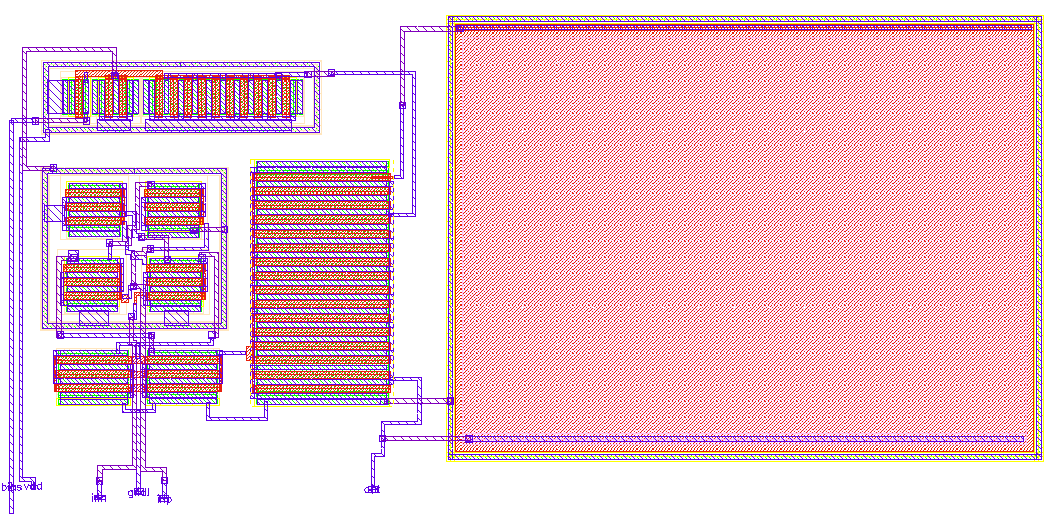
\includegraphics[scale=.4]{FIG/miller_amplifier_layout_routed.png}
  	\caption{manually routed layout of a miller amplifier}
	\label{fig:miller_amplifier_routed_layout}
\end{figure}

\section{Changes for Routing in the existing Applications}

\subsection{Plantage}

\subsubsection{Missing Data}
First of all, to actually route the placements some data was missing in Plantage. Although at some points the routing was already prepared, example given the net names were available, important information was not given. These include:
\begin{itemize}
\item actual dimensions of the modules
\item parameter of the technology
\item vias and routes
\item guard rings
\end{itemize}

In awareness of the necessary routing for every module a bigger area was defined for the placement. The additional space between the modules could then be used to route the placement. Unfortunately, the information about the actual dimension of the modules was lost through this step. Therefore I withdrawed these changes and added the possibility to define a minimum distance between all modules.

The technology rules are passed through by the ICFBInterface to Plantage. At least for the technology definitions of Austria Microsystems it is not necessary to convert these rules, as the same format is chosen. For other manufacturers a conversion might be necessary.

Previously, the vias and routes were not considered at all. The main information which is needed to route are the dimension of the vias on the different layers and the width for the routes. Actually there is no real width for a route, but a minimal width, which a route must have. Usually this width is used for the connections. Also the dimensions for the via must be caculated \nref{eq:via_dimension} and the generated routes and placed vias needed to be added to the output of Plantage, so that they can be shown in the GUI.

Beforehand, every pin consisted only of one rectangle, which is obviously not enough. This basic information was used to minimize the estimated net length for the placements. For real routing we need more complex possibilities to define pins, as for example the gate can be connected from both sides. Moreover it is not recommended to contact over the diffusion area. This will result in even more complex contact areas, as they could be split up in different parts. The definition of these areas is done by the user in the GUI and handed over to Plantage. The used format defines for every pin, which a module has, at least one contact area, but eventually a lot more. During the routing then the acutal contact area is selected based on a certain heuristic.

\subsection{ICFBInterface}
The GUI-part of this application also needed some adaptions. This work was mainly done by Martin Keßler and contained the following parts:

\begin{itemize}
\item possibility to define contact areas
\item displaying routes and vias
\item possibility to change algorithm settings
\end{itemize}	

\section{Overview of Routing Algorithms}
A really nice overview of the existing routing algorithms and the different approaches can be found in \cite[page 149 till 201]{springer:eda_analog_routing}. The more sophisticated routing algorithms described there are based on two basic algorithms:
\begin{itemize}
\item Maze Router
\item Line Router
\end{itemize}
These algorithms are so-called general purpose router, they can be used for global and detailed routing. To find out which type of algorithm may be appropiate in my case I will have a short look on the most important algorithms.

\subsection{Basic Routing Algorithms}
\subsubsection{Maze Router}
Another often used name for algorithm is Lee's algorithm. But whatever the name is, it is based on a grid, where the obstacles and pins can be filled in. Basically, this is the entire information, which is necessary for the router. Afterwards, a wave of numbers is started from one pin and if this wave reaches the target a possible routing is found \nref{fig:maze_router}. The router guarantees the shortest possible route and will find a route in all cases if it is possible \cite[p. 693]{kaufmann:electronic_design_automation}. All in all this is a very simple approach, but it has several drawbacks. First of all, it is quite slow and very memory consuming \cite[p. 693]{kaufmann:electronic_design_automation}, as a quite big matrix might be necessary. This memory consumption also relies heavily on the grid size, which raises the next question: How fine should be the grid? Those aren't problems which can not be solved. So, for example to attack the problem with the performance it is possible to transform the algorithm into the A*-Algorithm, which is actually just a modified maze router that prefers the shorter directions to the target. Also for the other problems there are solutions, which are mainly part of the more sophisticated routing algorithms.

\begin{figure}
	\centering
	\setlength{\unitlength}{0.282222229121mm}
\begin{picture}(500.0, 500.0)(0, -500.0)
  \put(0,-500.0){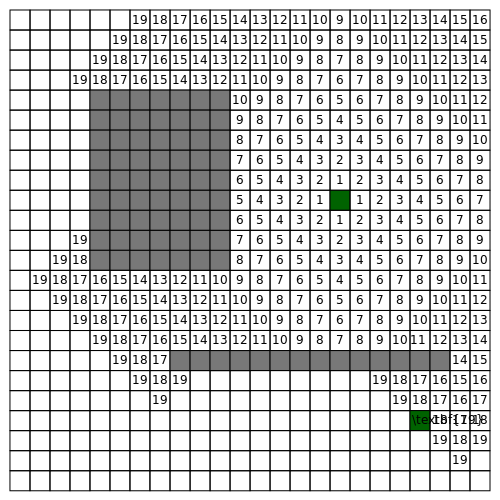
\includegraphics[height=141.11111456mm, width=141.11111456mm]{FIG/maze_router.svg.pdf}}
  \put(336.0,-184.0){\makebox(0,0)[l]{\smash{1}}}
  \put(356.0,-204.0){\makebox(0,0)[l]{\smash{1}}}
  \put(336.0,-224.0){\makebox(0,0)[l]{\smash{1}}}
  \put(316.0,-204.0){\makebox(0,0)[l]{\smash{1}}}
  \put(356.0,-224.0){\makebox(0,0)[l]{\smash{2}}}
  \put(376.0,-204.0){\makebox(0,0)[l]{\smash{2}}}
  \put(356.0,-184.0){\makebox(0,0)[l]{\smash{2}}}
  \put(316.0,-184.0){\makebox(0,0)[l]{\smash{2}}}
  \put(296.0,-204.0){\makebox(0,0)[l]{\smash{2}}}
  \put(316.0,-224.0){\makebox(0,0)[l]{\smash{2}}}
  \put(336.0,-164.0){\makebox(0,0)[l]{\smash{2}}}
  \put(336.0,-244.0){\makebox(0,0)[l]{\smash{2}}}
  \put(356.0,-244.0){\makebox(0,0)[l]{\smash{3}}}
  \put(376.0,-224.0){\makebox(0,0)[l]{\smash{3}}}
  \put(396.0,-204.0){\makebox(0,0)[l]{\smash{3}}}
  \put(376.0,-184.0){\makebox(0,0)[l]{\smash{3}}}
  \put(356.0,-164.0){\makebox(0,0)[l]{\smash{3}}}
  \put(336.0,-144.0){\makebox(0,0)[l]{\smash{3}}}
  \put(316.0,-164.0){\makebox(0,0)[l]{\smash{3}}}
  \put(296.0,-184.0){\makebox(0,0)[l]{\smash{3}}}
  \put(276.0,-204.0){\makebox(0,0)[l]{\smash{3}}}
  \put(296.0,-224.0){\makebox(0,0)[l]{\smash{3}}}
  \put(316.0,-244.0){\makebox(0,0)[l]{\smash{3}}}
  \put(336.0,-264.0){\makebox(0,0)[l]{\smash{3}}}
  \put(336.0,-284.0){\makebox(0,0)[l]{\smash{4}}}
  \put(356.0,-264.0){\makebox(0,0)[l]{\smash{4}}}
  \put(376.0,-244.0){\makebox(0,0)[l]{\smash{4}}}
  \put(396.0,-224.0){\makebox(0,0)[l]{\smash{4}}}
  \put(416.0,-204.0){\makebox(0,0)[l]{\smash{4}}}
  \put(396.0,-184.0){\makebox(0,0)[l]{\smash{4}}}
  \put(376.0,-164.0){\makebox(0,0)[l]{\smash{4}}}
  \put(356.0,-144.0){\makebox(0,0)[l]{\smash{4}}}
  \put(336.0,-124.0){\makebox(0,0)[l]{\smash{4}}}
  \put(316.0,-144.0){\makebox(0,0)[l]{\smash{4}}}
  \put(296.0,-164.0){\makebox(0,0)[l]{\smash{4}}}
  \put(276.0,-184.0){\makebox(0,0)[l]{\smash{4}}}
  \put(256.0,-204.0){\makebox(0,0)[l]{\smash{4}}}
  \put(276.0,-224.0){\makebox(0,0)[l]{\smash{4}}}
  \put(296.0,-244.0){\makebox(0,0)[l]{\smash{4}}}
  \put(316.0,-264.0){\makebox(0,0)[l]{\smash{4}}}
  \put(336.0,-304.0){\makebox(0,0)[l]{\smash{5}}}
  \put(356.0,-284.0){\makebox(0,0)[l]{\smash{5}}}
  \put(376.0,-264.0){\makebox(0,0)[l]{\smash{5}}}
  \put(396.0,-244.0){\makebox(0,0)[l]{\smash{5}}}
  \put(416.0,-224.0){\makebox(0,0)[l]{\smash{5}}}
  \put(436.0,-204.0){\makebox(0,0)[l]{\smash{5}}}
  \put(416.0,-184.0){\makebox(0,0)[l]{\smash{5}}}
  \put(396.0,-164.0){\makebox(0,0)[l]{\smash{5}}}
  \put(376.0,-144.0){\makebox(0,0)[l]{\smash{5}}}
  \put(356.0,-124.0){\makebox(0,0)[l]{\smash{5}}}
  \put(336.0,-104.0){\makebox(0,0)[l]{\smash{5}}}
  \put(316.0,-124.0){\makebox(0,0)[l]{\smash{5}}}
  \put(296.0,-144.0){\makebox(0,0)[l]{\smash{5}}}
  \put(276.0,-164.0){\makebox(0,0)[l]{\smash{5}}}
  \put(256.0,-184.0){\makebox(0,0)[l]{\smash{5}}}
  \put(236.0,-204.0){\makebox(0,0)[l]{\smash{5}}}
  \put(256.0,-224.0){\makebox(0,0)[l]{\smash{5}}}
  \put(276.0,-244.0){\makebox(0,0)[l]{\smash{5}}}
  \put(296.0,-264.0){\makebox(0,0)[l]{\smash{5}}}
  \put(316.0,-284.0){\makebox(0,0)[l]{\smash{5}}}
  \put(336.0,-324.0){\makebox(0,0)[l]{\smash{6}}}
  \put(356.0,-304.0){\makebox(0,0)[l]{\smash{6}}}
  \put(376.0,-284.0){\makebox(0,0)[l]{\smash{6}}}
  \put(396.0,-264.0){\makebox(0,0)[l]{\smash{6}}}
  \put(416.0,-244.0){\makebox(0,0)[l]{\smash{6}}}
  \put(436.0,-224.0){\makebox(0,0)[l]{\smash{6}}}
  \put(456.0,-204.0){\makebox(0,0)[l]{\smash{6}}}
  \put(436.0,-184.0){\makebox(0,0)[l]{\smash{6}}}
  \put(416.0,-164.0){\makebox(0,0)[l]{\smash{6}}}
  \put(396.0,-144.0){\makebox(0,0)[l]{\smash{6}}}
  \put(376.0,-124.0){\makebox(0,0)[l]{\smash{6}}}
  \put(356.0,-104.0){\makebox(0,0)[l]{\smash{6}}}
  \put(336.0,-84.0){\makebox(0,0)[l]{\smash{6}}}
  \put(316.0,-104.0){\makebox(0,0)[l]{\smash{6}}}
  \put(296.0,-124.0){\makebox(0,0)[l]{\smash{6}}}
  \put(276.0,-144.0){\makebox(0,0)[l]{\smash{6}}}
  \put(256.0,-164.0){\makebox(0,0)[l]{\smash{6}}}
  \put(236.0,-184.0){\makebox(0,0)[l]{\smash{6}}}
  \put(236.0,-224.0){\makebox(0,0)[l]{\smash{6}}}
  \put(256.0,-244.0){\makebox(0,0)[l]{\smash{6}}}
  \put(276.0,-264.0){\makebox(0,0)[l]{\smash{6}}}
  \put(296.0,-284.0){\makebox(0,0)[l]{\smash{6}}}
  \put(316.0,-304.0){\makebox(0,0)[l]{\smash{6}}}
  \put(336.0,-344.0){\makebox(0,0)[l]{\smash{7}}}
  \put(356.0,-324.0){\makebox(0,0)[l]{\smash{7}}}
  \put(376.0,-304.0){\makebox(0,0)[l]{\smash{7}}}
  \put(396.0,-284.0){\makebox(0,0)[l]{\smash{7}}}
  \put(416.0,-264.0){\makebox(0,0)[l]{\smash{7}}}
  \put(436.0,-244.0){\makebox(0,0)[l]{\smash{7}}}
  \put(456.0,-224.0){\makebox(0,0)[l]{\smash{7}}}
  \put(476.0,-204.0){\makebox(0,0)[l]{\smash{7}}}
  \put(456.0,-184.0){\makebox(0,0)[l]{\smash{7}}}
  \put(436.0,-164.0){\makebox(0,0)[l]{\smash{7}}}
  \put(416.0,-144.0){\makebox(0,0)[l]{\smash{7}}}
  \put(396.0,-124.0){\makebox(0,0)[l]{\smash{7}}}
  \put(376.0,-104.0){\makebox(0,0)[l]{\smash{7}}}
  \put(356.0,-84.0){\makebox(0,0)[l]{\smash{7}}}
  \put(336.0,-64.0){\makebox(0,0)[l]{\smash{7}}}
  \put(316.0,-84.0){\makebox(0,0)[l]{\smash{7}}}
  \put(296.0,-104.0){\makebox(0,0)[l]{\smash{7}}}
  \put(276.0,-124.0){\makebox(0,0)[l]{\smash{7}}}
  \put(256.0,-144.0){\makebox(0,0)[l]{\smash{7}}}
  \put(236.0,-164.0){\makebox(0,0)[l]{\smash{7}}}
  \put(236.0,-244.0){\makebox(0,0)[l]{\smash{7}}}
  \put(256.0,-264.0){\makebox(0,0)[l]{\smash{7}}}
  \put(276.0,-284.0){\makebox(0,0)[l]{\smash{7}}}
  \put(296.0,-304.0){\makebox(0,0)[l]{\smash{7}}}
  \put(316.0,-324.0){\makebox(0,0)[l]{\smash{7}}}
  \put(236.0,-264.0){\makebox(0,0)[l]{\smash{8}}}
  \put(256.0,-284.0){\makebox(0,0)[l]{\smash{8}}}
  \put(276.0,-304.0){\makebox(0,0)[l]{\smash{8}}}
  \put(296.0,-324.0){\makebox(0,0)[l]{\smash{8}}}
  \put(316.0,-344.0){\makebox(0,0)[l]{\smash{8}}}
  \put(356.0,-344.0){\makebox(0,0)[l]{\smash{8}}}
  \put(376.0,-324.0){\makebox(0,0)[l]{\smash{8}}}
  \put(396.0,-304.0){\makebox(0,0)[l]{\smash{8}}}
  \put(416.0,-284.0){\makebox(0,0)[l]{\smash{8}}}
  \put(436.0,-264.0){\makebox(0,0)[l]{\smash{8}}}
  \put(456.0,-244.0){\makebox(0,0)[l]{\smash{8}}}
  \put(476.0,-224.0){\makebox(0,0)[l]{\smash{8}}}
  \put(476.0,-184.0){\makebox(0,0)[l]{\smash{8}}}
  \put(456.0,-164.0){\makebox(0,0)[l]{\smash{8}}}
  \put(436.0,-144.0){\makebox(0,0)[l]{\smash{8}}}
  \put(416.0,-124.0){\makebox(0,0)[l]{\smash{8}}}
  \put(396.0,-104.0){\makebox(0,0)[l]{\smash{8}}}
  \put(376.0,-84.0){\makebox(0,0)[l]{\smash{8}}}
  \put(356.0,-64.0){\makebox(0,0)[l]{\smash{8}}}
  \put(336.0,-44.0){\makebox(0,0)[l]{\smash{8}}}
  \put(316.0,-64.0){\makebox(0,0)[l]{\smash{8}}}
  \put(296.0,-84.0){\makebox(0,0)[l]{\smash{8}}}
  \put(276.0,-104.0){\makebox(0,0)[l]{\smash{8}}}
  \put(256.0,-124.0){\makebox(0,0)[l]{\smash{8}}}
  \put(236.0,-144.0){\makebox(0,0)[l]{\smash{8}}}
  \put(236.0,-284.0){\makebox(0,0)[l]{\smash{9}}}
  \put(256.0,-304.0){\makebox(0,0)[l]{\smash{9}}}
  \put(276.0,-324.0){\makebox(0,0)[l]{\smash{9}}}
  \put(296.0,-344.0){\makebox(0,0)[l]{\smash{9}}}
  \put(376.0,-344.0){\makebox(0,0)[l]{\smash{9}}}
  \put(396.0,-324.0){\makebox(0,0)[l]{\smash{9}}}
  \put(416.0,-304.0){\makebox(0,0)[l]{\smash{9}}}
  \put(436.0,-284.0){\makebox(0,0)[l]{\smash{9}}}
  \put(456.0,-264.0){\makebox(0,0)[l]{\smash{9}}}
  \put(476.0,-244.0){\makebox(0,0)[l]{\smash{9}}}
  \put(476.0,-164.0){\makebox(0,0)[l]{\smash{9}}}
  \put(456.0,-144.0){\makebox(0,0)[l]{\smash{9}}}
  \put(436.0,-124.0){\makebox(0,0)[l]{\smash{9}}}
  \put(416.0,-104.0){\makebox(0,0)[l]{\smash{9}}}
  \put(396.0,-84.0){\makebox(0,0)[l]{\smash{9}}}
  \put(376.0,-64.0){\makebox(0,0)[l]{\smash{9}}}
  \put(356.0,-44.0){\makebox(0,0)[l]{\smash{9}}}
  \put(336.0,-24.0){\makebox(0,0)[l]{\smash{9}}}
  \put(316.0,-44.0){\makebox(0,0)[l]{\smash{9}}}
  \put(296.0,-64.0){\makebox(0,0)[l]{\smash{9}}}
  \put(276.0,-84.0){\makebox(0,0)[l]{\smash{9}}}
  \put(256.0,-104.0){\makebox(0,0)[l]{\smash{9}}}
  \put(236.0,-124.0){\makebox(0,0)[l]{\smash{9}}}
  \put(212.0,-284.0){\makebox(0,0)[l]{\smash{10}}}
  \put(232.0,-304.0){\makebox(0,0)[l]{\smash{10}}}
  \put(252.0,-324.0){\makebox(0,0)[l]{\smash{10}}}
  \put(272.0,-344.0){\makebox(0,0)[l]{\smash{10}}}
  \put(392.0,-344.0){\makebox(0,0)[l]{\smash{10}}}
  \put(412.0,-324.0){\makebox(0,0)[l]{\smash{10}}}
  \put(432.0,-304.0){\makebox(0,0)[l]{\smash{10}}}
  \put(452.0,-284.0){\makebox(0,0)[l]{\smash{10}}}
  \put(472.0,-264.0){\makebox(0,0)[l]{\smash{10}}}
  \put(472.0,-144.0){\makebox(0,0)[l]{\smash{10}}}
  \put(452.0,-124.0){\makebox(0,0)[l]{\smash{10}}}
  \put(432.0,-104.0){\makebox(0,0)[l]{\smash{10}}}
  \put(412.0,-84.0){\makebox(0,0)[l]{\smash{10}}}
  \put(392.0,-64.0){\makebox(0,0)[l]{\smash{10}}}
  \put(372.0,-44.0){\makebox(0,0)[l]{\smash{10}}}
  \put(352.0,-24.0){\makebox(0,0)[l]{\smash{10}}}
  \put(312.0,-24.0){\makebox(0,0)[l]{\smash{10}}}
  \put(292.0,-44.0){\makebox(0,0)[l]{\smash{10}}}
  \put(272.0,-64.0){\makebox(0,0)[l]{\smash{10}}}
  \put(252.0,-84.0){\makebox(0,0)[l]{\smash{10}}}
  \put(232.0,-104.0){\makebox(0,0)[l]{\smash{10}}}
  \put(192.0,-284.0){\makebox(0,0)[l]{\smash{11}}}
  \put(212.0,-304.0){\makebox(0,0)[l]{\smash{11}}}
  \put(232.0,-324.0){\makebox(0,0)[l]{\smash{11}}}
  \put(252.0,-344.0){\makebox(0,0)[l]{\smash{11}}}
  \put(410.0,-344.0){\makebox(0,0)[l]{\smash{11}}}
  \put(432.0,-324.0){\makebox(0,0)[l]{\smash{11}}}
  \put(452.0,-304.0){\makebox(0,0)[l]{\smash{11}}}
  \put(472.0,-284.0){\makebox(0,0)[l]{\smash{11}}}
  \put(472.0,-124.0){\makebox(0,0)[l]{\smash{11}}}
  \put(452.0,-104.0){\makebox(0,0)[l]{\smash{11}}}
  \put(432.0,-84.0){\makebox(0,0)[l]{\smash{11}}}
  \put(412.0,-64.0){\makebox(0,0)[l]{\smash{11}}}
  \put(392.0,-44.0){\makebox(0,0)[l]{\smash{11}}}
  \put(372.0,-24.0){\makebox(0,0)[l]{\smash{11}}}
  \put(292.0,-24.0){\makebox(0,0)[l]{\smash{11}}}
  \put(272.0,-44.0){\makebox(0,0)[l]{\smash{11}}}
  \put(252.0,-64.0){\makebox(0,0)[l]{\smash{11}}}
  \put(232.0,-84.0){\makebox(0,0)[l]{\smash{11}}}
  \put(172.0,-284.0){\makebox(0,0)[l]{\smash{12}}}
  \put(192.0,-304.0){\makebox(0,0)[l]{\smash{12}}}
  \put(212.0,-324.0){\makebox(0,0)[l]{\smash{12}}}
  \put(232.0,-344.0){\makebox(0,0)[l]{\smash{12}}}
  \put(432.0,-344.0){\makebox(0,0)[l]{\smash{12}}}
  \put(452.0,-324.0){\makebox(0,0)[l]{\smash{12}}}
  \put(472.0,-304.0){\makebox(0,0)[l]{\smash{12}}}
  \put(472.0,-104.0){\makebox(0,0)[l]{\smash{12}}}
  \put(452.0,-84.0){\makebox(0,0)[l]{\smash{12}}}
  \put(432.0,-64.0){\makebox(0,0)[l]{\smash{12}}}
  \put(412.0,-44.0){\makebox(0,0)[l]{\smash{12}}}
  \put(392.0,-24.0){\makebox(0,0)[l]{\smash{12}}}
  \put(272.0,-24.0){\makebox(0,0)[l]{\smash{12}}}
  \put(252.0,-44.0){\makebox(0,0)[l]{\smash{12}}}
  \put(232.0,-64.0){\makebox(0,0)[l]{\smash{12}}}
  \put(212.0,-84.0){\makebox(0,0)[l]{\smash{12}}}
  \put(152.0,-284.0){\makebox(0,0)[l]{\smash{13}}}
  \put(172.0,-304.0){\makebox(0,0)[l]{\smash{13}}}
  \put(192.0,-324.0){\makebox(0,0)[l]{\smash{13}}}
  \put(212.0,-344.0){\makebox(0,0)[l]{\smash{13}}}
  \put(452.0,-344.0){\makebox(0,0)[l]{\smash{13}}}
  \put(472.0,-324.0){\makebox(0,0)[l]{\smash{13}}}
  \put(472.0,-84.0){\makebox(0,0)[l]{\smash{13}}}
  \put(452.0,-64.0){\makebox(0,0)[l]{\smash{13}}}
  \put(432.0,-44.0){\makebox(0,0)[l]{\smash{13}}}
  \put(412.0,-24.0){\makebox(0,0)[l]{\smash{13}}}
  \put(252.0,-24.0){\makebox(0,0)[l]{\smash{13}}}
  \put(232.0,-44.0){\makebox(0,0)[l]{\smash{13}}}
  \put(212.0,-64.0){\makebox(0,0)[l]{\smash{13}}}
  \put(192.0,-84.0){\makebox(0,0)[l]{\smash{13}}}
  \put(132.0,-284.0){\makebox(0,0)[l]{\smash{14}}}
  \put(152.0,-304.0){\makebox(0,0)[l]{\smash{14}}}
  \put(172.0,-324.0){\makebox(0,0)[l]{\smash{14}}}
  \put(192.0,-344.0){\makebox(0,0)[l]{\smash{14}}}
  \put(452.0,-364.0){\makebox(0,0)[l]{\smash{14}}}
  \put(472.0,-344.0){\makebox(0,0)[l]{\smash{14}}}
  \put(472.0,-64.0){\makebox(0,0)[l]{\smash{14}}}
  \put(452.0,-44.0){\makebox(0,0)[l]{\smash{14}}}
  \put(432.0,-24.0){\makebox(0,0)[l]{\smash{14}}}
  \put(232.0,-24.0){\makebox(0,0)[l]{\smash{14}}}
  \put(212.0,-44.0){\makebox(0,0)[l]{\smash{14}}}
  \put(192.0,-64.0){\makebox(0,0)[l]{\smash{14}}}
  \put(172.0,-84.0){\makebox(0,0)[l]{\smash{14}}}
  \put(112.0,-284.0){\makebox(0,0)[l]{\smash{15}}}
  \put(132.0,-304.0){\makebox(0,0)[l]{\smash{15}}}
  \put(152.0,-324.0){\makebox(0,0)[l]{\smash{15}}}
  \put(172.0,-344.0){\makebox(0,0)[l]{\smash{15}}}
  \put(472.0,-364.0){\makebox(0,0)[l]{\smash{15}}}
  \put(452.0,-384.0){\makebox(0,0)[l]{\smash{15}}}
  \put(472.0,-44.0){\makebox(0,0)[l]{\smash{15}}}
  \put(452.0,-24.0){\makebox(0,0)[l]{\smash{15}}}
  \put(212.0,-24.0){\makebox(0,0)[l]{\smash{15}}}
  \put(192.0,-44.0){\makebox(0,0)[l]{\smash{15}}}
  \put(172.0,-64.0){\makebox(0,0)[l]{\smash{15}}}
  \put(152.0,-84.0){\makebox(0,0)[l]{\smash{15}}}
  \put(92.0,-284.0){\makebox(0,0)[l]{\smash{16}}}
  \put(112.0,-304.0){\makebox(0,0)[l]{\smash{16}}}
  \put(132.0,-324.0){\makebox(0,0)[l]{\smash{16}}}
  \put(152.0,-344.0){\makebox(0,0)[l]{\smash{16}}}
  \put(432.0,-384.0){\makebox(0,0)[l]{\smash{16}}}
  \put(472.0,-384.0){\makebox(0,0)[l]{\smash{16}}}
  \put(452.0,-404.0){\makebox(0,0)[l]{\smash{16}}}
  \put(472.0,-24.0){\makebox(0,0)[l]{\smash{16}}}
  \put(192.0,-24.0){\makebox(0,0)[l]{\smash{16}}}
  \put(172.0,-44.0){\makebox(0,0)[l]{\smash{16}}}
  \put(152.0,-64.0){\makebox(0,0)[l]{\smash{16}}}
  \put(132.0,-84.0){\makebox(0,0)[l]{\smash{16}}}
  \put(72.0,-284.0){\makebox(0,0)[l]{\smash{17}}}
  \put(92.0,-304.0){\makebox(0,0)[l]{\smash{17}}}
  \put(112.0,-324.0){\makebox(0,0)[l]{\smash{17}}}
  \put(132.0,-344.0){\makebox(0,0)[l]{\smash{17}}}
  \put(152.0,-364.0){\makebox(0,0)[l]{\smash{17}}}
  \put(412.0,-384.0){\makebox(0,0)[l]{\smash{17}}}
  \put(432.0,-404.0){\makebox(0,0)[l]{\smash{17}}}
  \put(452.0,-424.0){\makebox(0,0)[l]{\smash{17}}}
  \put(472.0,-404.0){\makebox(0,0)[l]{\smash{17}}}
  \put(172.0,-24.0){\makebox(0,0)[l]{\smash{17}}}
  \put(152.0,-44.0){\makebox(0,0)[l]{\smash{17}}}
  \put(132.0,-64.0){\makebox(0,0)[l]{\smash{17}}}
  \put(112.0,-84.0){\makebox(0,0)[l]{\smash{17}}}
  \put(72.0,-264.0){\makebox(0,0)[l]{\smash{18}}}
  \put(52.0,-284.0){\makebox(0,0)[l]{\smash{18}}}
  \put(72.0,-304.0){\makebox(0,0)[l]{\smash{18}}}
  \put(92.0,-324.0){\makebox(0,0)[l]{\smash{18}}}
  \put(112.0,-344.0){\makebox(0,0)[l]{\smash{18}}}
  \put(132.0,-364.0){\makebox(0,0)[l]{\smash{18}}}
  \put(152.0,-384.0){\makebox(0,0)[l]{\smash{18}}}
  \put(392.0,-384.0){\makebox(0,0)[l]{\smash{18}}}
  \put(412.0,-404.0){\makebox(0,0)[l]{\smash{18}}}
  \put(432.0,-424.0){\makebox(0,0)[l]{\smash{18}}}
  \put(452.0,-444.0){\makebox(0,0)[l]{\smash{18}}}
  \put(472.0,-424.0){\makebox(0,0)[l]{\smash{18}}}
  \put(152.0,-24.0){\makebox(0,0)[l]{\smash{18}}}
  \put(132.0,-44.0){\makebox(0,0)[l]{\smash{18}}}
  \put(112.0,-64.0){\makebox(0,0)[l]{\smash{18}}}
  \put(92.0,-84.0){\makebox(0,0)[l]{\smash{18}}}
  \put(132.0,-24.0){\makebox(0,0)[l]{\smash{19}}}
  \put(112.0,-44.0){\makebox(0,0)[l]{\smash{19}}}
  \put(92.0,-64.0){\makebox(0,0)[l]{\smash{19}}}
  \put(72.0,-84.0){\makebox(0,0)[l]{\smash{19}}}
  \put(72.0,-244.0){\makebox(0,0)[l]{\smash{19}}}
  \put(52.0,-264.0){\makebox(0,0)[l]{\smash{19}}}
  \put(32.0,-284.0){\makebox(0,0)[l]{\smash{19}}}
  \put(52.0,-304.0){\makebox(0,0)[l]{\smash{19}}}
  \put(72.0,-324.0){\makebox(0,0)[l]{\smash{19}}}
  \put(92.0,-344.0){\makebox(0,0)[l]{\smash{19}}}
  \put(112.0,-364.0){\makebox(0,0)[l]{\smash{19}}}
  \put(132.0,-384.0){\makebox(0,0)[l]{\smash{19}}}
  \put(152.0,-404.0){\makebox(0,0)[l]{\smash{19}}}
  \put(172.0,-384.0){\makebox(0,0)[l]{\smash{19}}}
  \put(372.0,-384.0){\makebox(0,0)[l]{\smash{19}}}
  \put(392.0,-404.0){\makebox(0,0)[l]{\smash{19}}}
  \put(412.0,-424.0){\makebox(0,0)[l]{\smash{\textbf{19}}}}
  \put(432.0,-444.0){\makebox(0,0)[l]{\smash{19}}}
  \put(472.0,-444.0){\makebox(0,0)[l]{\smash{19}}}
  \put(452.0,-464.00002){\makebox(0,0)[l]{\smash{19}}}
\end{picture}
	\caption{a wavefront explores the area till it reaches the target}
	\label{fig:maze_router}
\end{figure}

\subsubsection{Line Router}
The main difference from a line router to a maze router is the usage of lines as part of a route instead of points. This improves the memory usage and usually also avoids unnecessary bends. At the same time this modification causes the loss of the guarantee to find the shortest path \cite[p. 695]{kaufmann:electronic_design_automation}. The other big difference lies in the search algorithm itself, as the line router performs a depth-first search instead of a breadth-first search like the maze router. The basic idea behind this type of router is to try to reach the target, or at least one of its coordinates in the first step, through an as long as possible line. This line may hit an obstacle, which means that the direction must be changed. And in this way the router always goes as far as possible into a direction and changes the direction till he reaches the target.

\subsection{Steiner Routing}
\label{subsec:steiner_routing}
The algorithms above only considered two-pin nets, but very often nets have more than two pins. For these cases a possible solution would be to consider only two pins at a time and connect the others sequentially to the previous ones. This can result in a lot worse results than the optimum \cite[p. 701]{kaufmann:electronic_design_automation}. A better approach is to use a Steiner-tree \cite[page 153]{springer:eda_analog_routing}.

\subsection{Sophisticated Routing Algorithms}
As it is not the topic of this thesis to describe in detail every possible routing algorithm I just want to bring up here some possible approaches. They are built around several very nice ideas but had all one drawback, which made them not useful for the hierarchical placer, or were a bit to complex to be easy to implement. As the target of this thesis is mainly to create feasible and useful, but not perfect, layouts, I haven't chosen one of these sophisticated algorithms.
\begin{itemize}
\item ROSA \cite[page 165]{springer:eda_analog_routing}
\item MIGHTY \cite[page 166]{springer:eda_analog_routing}
\item ILAC \cite[page 167]{springer:eda_analog_routing}
\item SALIM \cite[page 167]{springer:eda_analog_routing}
\item SLAM \cite[page 167]{springer:eda_analog_routing}
\item hierarchical global router \cite[page 168]{springer:eda_analog_routing}
\item plan-based layout algorithm \cite[page 168]{springer:eda_analog_routing}
\item ANAGRAM \cite[page 168]{springer:eda_analog_routing}
\item ANAGRAM II \cite[page 168]{springer:eda_analog_routing}
\item area router \cite[page 168]{springer:eda_analog_routing}
\item modified Lee's algorithm \cite[page 170]{springer:eda_analog_routing}
\item ROAD \cite[page 170]{springer:eda_analog_routing}
\item ANAGRAM III \cite[page 170]{springer:eda_analog_routing}
\item router with constraint generator \cite[page 172]{springer:eda_analog_routing}
\end{itemize}

\subsection{Routing algorithms integrated into the placer}
It could be a very good idea to try to integrate the routing into the placer. Possible approaches into this direction are KOAN \cite[page 178]{springer:eda_analog_routing}, RACHANA \cite[page 178]{springer:eda_analog_routing}, GELSA \cite[page 179]{springer:eda_analog_routing}, and several others. The major problem with these solutions is the big modification of the placer. Actually it is quite useless to try to integrate the routing algorithm this way afterwards into a placer, as it must be created for this case with the routing in mind from the beginning. As the placer in Plantage wasn't supposed to include the routing algorithm, I had to use a different approach.

\subsection{Template Based Algorithms}
Template based algorithms do not start from scratch, they already have a possible layout for a slightly different circuit or technology. Such a solution can be used in several cases and gives the layout designer nearly full control over the process. In my case I have to assume that there is no such template available and the intention of the whole set of tools would be that the user has to provide as less information as possible. This would really mean \textit{electronic design \textbf{automation}} and therefore should be the real target.

\section{Implemented Routing Algorithms}
\label{sec:implemented_algorithms}
My first decision to make was to decide which algorithms I should implement. The more sophisticated solutions and all global and detailed approaches seemed a bit to complex to implement them clean in only a few weeks. So the real choice was to use something based on a maze or a line router. As the line routers seemed to be a good trade-off between complexity and performance I've chosen something based on them. In the end I've implemented three different routing algorithms: first of all a typical line expansion router. This solutions doesn't consider all constraints but it is able to create at least reasonable results. Afterwards this algorithm was extended to consider additional constraints. To improve the performance I also implemented a very special version of the line expansion router, which really only creates feasible, but not very useful routings. This router can be used for the pre-routing, where the results are not stored anyway.

\subsection{Line Expansion Router}

\subsubsection{Select a Target}
The first thing which the algorithm has to do before it can calculate a route is to select the start and target contact area. There can be several possibilities, as every pin can have several contact areas. Later on we will even see that already created routes can be candidates to start or end with a route. Basically, this task can be seen as the selection of the closest rectangles of two lists of possibilities. For this I first want to talk a little bit about how the closest distance between two rectangles can be calculated.

For two rectangles there are several possible constellations. The first one I check is if they overlap. If this is the case I can calculate easily the rectangle which is covered by both \nref{fig:rectangles_overlapping} and the distance is 0. As start points for both rectangles I can select the center of gravity of the overlapping area.

\begin{figure}
	\centering
	\setlength{\unitlength}{0.282222229121mm}
\begin{picture}(275.80054, 174.07812)(0, -174.07812)
  \put(0,-174.07812){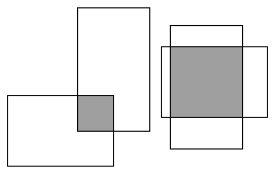
\includegraphics[height=49.1287150676mm, width=77.8370431916mm]{FIG/rectangles_overlapping.svg.pdf}}
\end{picture}
  	\caption{overlapping area of two rectangles is again a rectangle}
	\label{fig:rectangles_overlapping}
\end{figure}

If the two rectangles do not overlap it becomes a little bit more difficult. In this case I can at least say that one of the rectangle has its closest point at one of the edges. Actually, there can be even an endless count of solutions for this problem, but I'm only interested in one of them. Because of this I select the easiest to calculate solution, which means the selection of a corner for one rectangle. The closest corner from the first rectangle to the second one is that one, which has the closest euclidean distance to the center of gravity of the second one \nref{fig:rectangles_closest_corner}. As the closest point of the first rectangle is now known, I can start to select the closest point on the second one. This point must be obviously on one of the edges. Every edge is basically a line segment, where the closest point can be calculated easily. For this task I first need the expansion of the line segment into a whole line. I then can turn this line 90 degrees (it doesn't matter in which direction as it is a line) and move this new line, so that it crosses the point, from which I want to know the closest point on the line segment. The crossing point of these two lines if it is also inside the line segment is the closest point. If this crossing point is outside the line segment, the closest point must be the start or end point of the line segment, which are actually the rectangle's corners.

\begin{figure}
	\centering
	\setlength{\unitlength}{0.282222229121mm}
\begin{picture}(275.80054, 174.07812)(0, -174.07812)
  \put(0,-174.07812){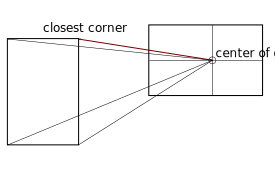
\includegraphics[height=49.1287150676mm, width=77.8370431916mm]{FIG/rectangles_closest_corner.svg.pdf}}
  \put(216.142843,-57.22096){\makebox(0,0)[l]{\smash{center of gravity}}}
  \put(43.019685,-31.84584){\makebox(0,0)[l]{\smash{closest corner}}}
\end{picture}
  	\caption{the closest corner is that one, which has the smallest distance to the center of gravity of the other one}
	\label{fig:rectangles_closest_corner}
\end{figure}

\subsubsection{Consider Obstacles}
After the algorithm has selected start and target contact areas the next step is to avoid routes across modules. For this purpose during all the following steps the modules are considered as obstacles. But during the first step usually the route has first to get out of the module. To avoid additional, accidentally added, gates the algorithm has to choose the shortest way to get out of the module. To avoid problems with the design rules it is not possible to start right at the contact area to the next layer and use for example metal to get out of the module as fast as possible.

As the algorithm now has all the necessary information the actual line expansion routing can start. The main idea behind a line expansion router is that the routes are created sequentially. Every single step is based on a map of obstacles, which the route mustn't cross. From the starting point beginning I always calculate the next possible point of a route and apply the same algorithm afterwards again to this partial problem. At the beginning of this recursive algorithm, as usual, I check the terminating condition if I have reached the target point.

In every single step I have to make several decisions: First I group the possible directions in good and bad directions \nref{fig:router_good_bad_direction}. Good directions are those, which reduce the distance to the target, whereas bad ones are all the others.

\begin{figure}
	\centering
	\setlength{\unitlength}{0.282222229121mm}
\begin{picture}(322.55502, 271.89285)(0, -271.89285)
  \put(0,-271.89285){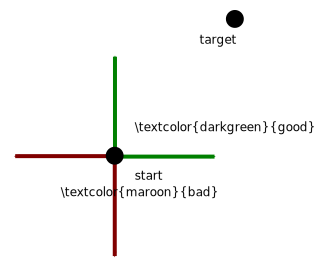
\includegraphics[height=76.7342062091mm, width=91.0321967586mm]{FIG/router_good_bad_direction.svg.pdf}}
  \put(134.88118,-180.46426){\makebox(0,0)[l]{\smash{start}}}
  \put(60.59547,-196.89285){\makebox(0,0)[l]{\smash{\textcolor{maroon}{bad}}}}
  \put(134.88118,-131.80496){\makebox(0,0)[l]{\smash{\textcolor{darkgreen}{good}}}}
  \put(199.88118,-43.8779){\makebox(0,0)[l]{\smash{target}}}
\end{picture}
  	\caption{good and bad directions}
	\label{fig:router_good_bad_direction}
\end{figure}

Additionally, it makes no sense to go back the same direction where the last step came from. Also the same direction like the last step is not reasonable. The reason therefore is that if this would be a good decision, the last step could have gone further. So I remove these two directions from the good directions. After this selection I can make one step further in every good directon, as far as possible. This means that the next step can go as far as no obstacle is on the way or the target (in this coordinate) is reached \nref{fig:router_go_as_far_as_possible}.

\begin{figure}
	\centering
	\subfloat[no obstacle]{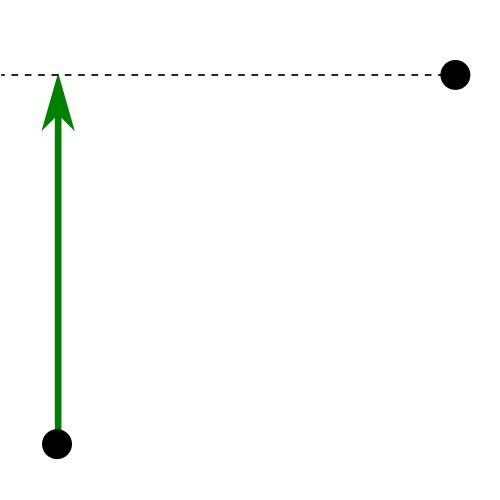
\includegraphics[scale=0.8]{FIG/router_as_far_as_possible.png}}
	\subfloat[with obstacle]{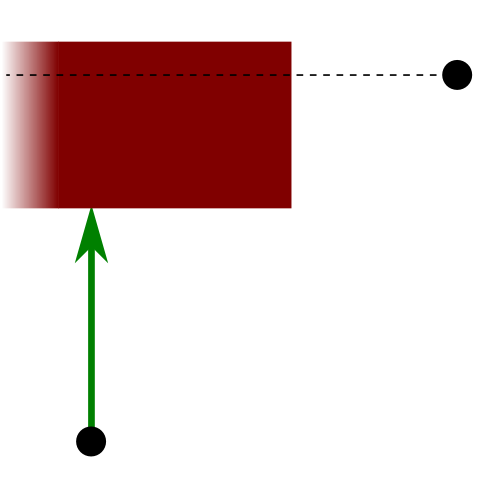
\includegraphics[scale=0.8]{FIG/router_as_far_as_possible_obstacle.png}}
	\caption{in a good direction the route can go as far as possible}
	\label{fig:router_go_as_far_as_possible}
\end{figure}


During the calculation of the steps towards the target I count those, which are feasible. If none of them is feasible I will have to select one of the bad directions for the next step. A major premission for this is also that the last step ended at an obstacle. The router now can go as far as necessary into this bad direction \nref{fig:router_as_far_as_necessary}.

\begin{figure}
	\centering
	\setlength{\unitlength}{0.282222229121mm}
\begin{picture}(500.0, 300.0)(0, -300.0)
  \put(0,-300.0){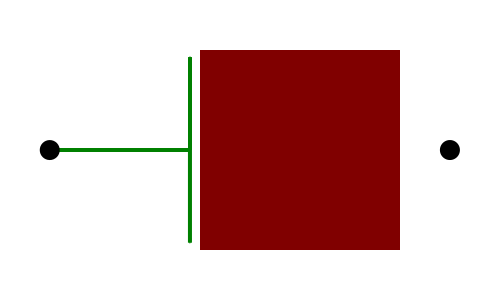
\includegraphics[height=84.6666687363mm, width=141.11111456mm]{FIG/router_as_far_as_necessary.svg.pdf}}
\end{picture}
 	\caption{a step into a bad direction should go only as far as necessary}
	\label{fig:router_as_far_as_necessary}
\end{figure}

Last but no least it is also possible to switch to the neighboured layers. For modules the obstacle can not be crossed with this way, as they are obstacles at every layer. But if for example the obstacle is just another route a layer switch may solve the problem.

\subsubsection{Avoid Collisions}
To avoid collisions I take into account the preferred directions for every layer. This information is again stored in the technology file and describes if a layer should be used for horziontal or vertical routes. This reduces the possibility of collisions very efficiently and results in less complex layouts.

\subsubsection{Symmetric Routes}
In manually created layouts an usual way to route symmetric elements is to create them optical symmetric. This optical symmetry gives the designer an easy way to create symmetry. But the really important part about routing symmetries is to match the parasitics. The resistance of the route is for sure matched for the symmetric routes through an optical symmetry, but the capacitive couplings are obeyed in most cases. Therefore I concentrated on the resistance. To also consider the capacities it would have been necessary to create all routes at the same time. Only with such an approach I can evaluate the capacitive parasitics, otherwise I never know what influence routes created afterwards will have. As I have chosen to create the routes one by one I can't consider the capacities for the symmetries.

But before I go more into detail of the routing I want to explain the situation a bit more. Symmetries are caused by symmetry constraints, which can have, as already described earlier \nref{subsec:symmetry_constraint}, single and pair modules. Single modules are quite useless for a symmetric routing. The only modules of interest are pair modules, no matter if they must be connected only together or also to another module.

In the routing I first extract all modules, which are symmetric and where both parts of the symmetry pair must be connected to the same net. Afterwards I connect these pairs together and the only possible start or end point for other routes is then the middle of the route between the pair. In this case the middle doesn't has to mean the same distance to both sides, but the same resistance to both modules. Therefore if for instance the route uses different layers from the modules to the middle, it is possible that the middle in terms of resistance can be different to the middle in terms of distance.

\subsubsection{Guard Rings}
With guards \nref{fig:guard_ring} a designer can protect for example a certain signal from another very noisy one or protect whole module groups. The latter one is often used for current mirrors, as they are very sensitive against noise. In physical representation a guard or guard ring is only a layer, for instance MET1, contacted to the substrate and connected to a certain Voltage level (often ground). For the routing this results only in an additional obstacle on this layer.

\begin{figure}
	\centering
	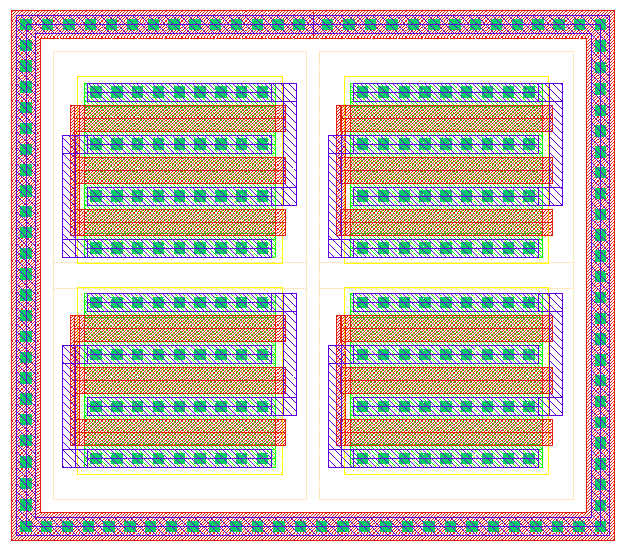
\includegraphics[scale=.6]{FIG/guard_ring.png}
  	\caption{the common centroid of a differential pair, protected from noise by a guard ring}
	\label{fig:guard_ring}
\end{figure}

The major difference of guard rings to usual obstacles is that they are obstacles only for certain nets. Or if you look at it the other way round, a guard ring isn't an obstacle for the nets inside. This is necessary so that other routes do not use the space inside a guard ring, but the pins inside can still be connected. For example a MET1-guard will result in a normal obstacle, for all nets, on MET1. On all other routing layers there will be also obstacles, but only for nets which don't have pins inside the guard ring.

\subsubsection{Multi-Pin Nets}
To solve the problem of multi-pin nets it would be possible to use a Steiner-tree \nref{subsec:steiner_routing}, but this approach wouldn't really be the easiest one to implement. That is why I've chosen a different solution. Basically, I connect at the beginnging the first two pins, where the order of the pins is random (actually they are sorted by there name alphabetically, but this was no intention and doesn't really matter). Afterwards I transform the whole new connection into additional possible targets. From this now bigger list of possible targets I select the closest one and connect the next pin to it. The result of this step is again transformed into additional targets for the next pin, and so on.

\subsubsection{Select a Route}
Finally, if the start point is the same as the end point I have to calculate a feasible and complete route. I add the result to all the possible routes for this necessary connection. From these routes the first, quite simple, algorithm chooses only the best one. As this algorithm calculates the routes sequentially it has no information about for example capacitive couplings, therefore the \emph{best} possibility is chosen on the lowest resistance.

For this first algorithm a lot of different variants for every necessary connection is quite a lot of information as it chooses only the shortest one in terms of resistance. But the results, which I generate here, can be reused for the extended version of the line expansion algorithm.

PICTURE MISSING OF ROUTED MILLER AMPLIFIER (LAYOUT)

\subsection{Line Expansion Feasibility Router}
In this special case I had to implement the routing into the hierarchical placing algorithm. This creates some additional requirements for the routing algorithms. The most important difference to an usual placer is that the actual positions of a module can change. Because of this, the positions are even not stored, only the selected variants and the enumeration sequence is used to specify a certain placement. As the positions of the routes would be relative to the module positions it is not really useful to store the routing results for the next higher hierarchy level. Another reason for this is the possibility of other modules, which could overlap with routes after the calculation of the placement on the next higher level. It is still important to try to route the placement, as a placement may cause very long or even infeasible routes. Because of these special requirements it is possible to select a different router for the pre-routing step than for the final routing. Actually, it would be possible to select every router here, but it is only reasonable to select one which requires less computing time.

This is the point where the line expansion feasibility router comes into play. This algorithm is a modified version of the basic line expansion algorithm. The only difference  is the amount of possible routes which are created for every necessary connection. The basic version creates as much as possible and the modified version only one route. This will result in usually quite bad layouts, and because of this the router shouldn't be used for the final step. But as pre router the algorithm is quite useful, as it is very fast and can select very efficient if a placement is at least feasible to route for a line expansion router.

\subsection{Extended Line Expansion Router}
This extended version of the line expansion router is based on the simple version. So it is again a sequential approach with the same drawbacks and advantages as the previous versions. The main difference to it is how I select the routes. I create the routes actually in the same way like for the previous version. To improve the performance I make a pre-selection based on the resistance, which can be done easily, as the routes are already sorted by there resistance. For all the routes, which are then left, I calculate the total edge and area capacity that would turn out, if this route is added to the connections of the previously routed nets. I then combine these values together to the parasitic sum
\[p = w_R \cdot R + w_{C_a} \cdot C_a + w_{C_e} \cdot C_e\]
(where $w_i$ are the weights and $R$, $C_a$ and $C_e$ are the parasitics as defined in \nref{sec:electrical_rules}) on which the actual selection is based.

PICTURE MISSING OF ROUTED MILLER AMPLIFIER (LAYOUT)